\documentclass[11pt]{article}
\usepackage[margin=1in]{geometry}
\usepackage{amsmath,amssymb,graphicx,booktabs,hyperref,xcolor}
\usepackage{siunitx}
\hypersetup{colorlinks=true,linkcolor=blue,urlcolor=blue}
\newcommand{\repl}{\textcolor{green!55!black}{\textbf{REPRODUCED}}}
\newcommand{\part}{\textcolor{orange!85!black}{\textbf{PARTIAL}}}
\newcommand{\oos}{\textcolor{gray}{\textbf{OUT-OF-SCOPE}}}
\title{Replication Report: \\ \emph{Multipole fluctuation theory for heavy fermion
systems: Application to multipole orders in CeB$_6$}\\ \small (Tazai \& Kontani, arXiv:1901.06213, 2019)}
\author{Automated replication (RPA core + analytic vertex-correction scaling)}
\date{2026-07-19}
\begin{document}
\maketitle

\begin{abstract}
We replicate the tractable core of Tazai \& Kontani's multipole-fluctuation theory for
the heavy-fermion compound CeB$_6$. From the Supplemental-Material Hamiltonian we
reconstruct the 2D periodic Anderson model (PAM), build all sixteen $\Gamma_8$-quartet
multipole operators in the $\sigma\!\otimes\!\tau$ pseudospin$\times$orbital basis,
compute the bare susceptibility bubble $\chi^0_Q(q)$, and form the channel-diagonal RPA
multipole susceptibilities using the paper's reported normalized Coulomb couplings
$U_0^Q$ (TABLE~II). We confirm the paper's \textbf{central RPA claim}: magnetic
(odd-rank) fluctuations dominate ($\alpha_{\rm mag}\!>\!\alpha_{\rm el}$; $\chi^{\rm
RPA}_{J_z}$ is $\sim\!40\times$ $\chi^{\rm RPA}_{O_{xy}}$), and the quadrupole channel
stays subcritical purely because $U_0^{O_{xy}}\!<\!U_0^{J_z}$. We further verify the
paper's analytic vertex-correction scaling $X^{\rm AL}\!\propto\!\xi^{4-d}$ (recovered
to $<2\%$ in $d=1,2,3$) and $X^{\rm MT}\!\sim\!\log\xi$, establishing why the
Aslamazov--Larkin (AL) vertex correction dominates the Maki--Thompson (MT) one near
magnetic criticality --- the mechanism the paper invokes for quadrupole order. The full
16$\times$16 two-loop AL/MT momentum integrals that yield the quantitative
$\chi_{O_{xy}}$ enhancement are marked out-of-scope for this run.
\end{abstract}

\section{Paper summary}
CeB$_6$ shows antiferro-quadrupole ($O_{xy}$) order at $T_Q=3.2$~K above magnetic order
($T_N=2.4$~K) and field-induced octupole ($T_{xyz}$) order. In an itinerant $f$-electron
picture the RPA of a PAM gives only magnetic (odd-rank) fluctuations; even-rank
(quadrupole) ones stay small. The authors add Aslamazov--Larkin (AL) vertex corrections
and show that interference between $(T_x,T_y)$ magnetic-multipole fluctuations enhances
$\chi_{O_{xy}}$ until it becomes the largest susceptibility, driving the antiferro-$O_{xy}$
order. A Zeeman field mixes $O_{xy}$ and $T_{xyz}$ (same IR $\Gamma_4$) and explains
field-induced octupole order.

\section{Model reconstructed (Supplemental Material A/B)}
Conduction band (Eq.~S1), 2D, $k_z=0$:
\begin{align*}
\varepsilon_k =\;& t_1(\cos k_x{+}\cos k_y)
+ t_2[\cos(k_x{+}k_y){+}\cos(k_x{-}k_y)]
+ t_3(\cos 2k_x{+}\cos 2k_y)\\
&+ t_4[\cos(2k_x{+}k_y){+}\cos(2k_x{-}k_y){+}\cos(2k_y{+}k_x){+}\cos(2k_y{-}k_x)]\\
&+ t_5[\cos(2k_x{+}2k_y){+}\cos(2k_x{-}2k_y)] + E_0,
\end{align*}
with $(t_1,\dots,t_5)=(-0.5,-0.889,0.292,-0.229,0.687)$, $E_0=1.33$, energy unit
$2|t_1|=1$. Hybridization (Eq.~S2): $V_{k f_1\uparrow}=-A_1 t_{sf}(\sin k_y - i\sin k_x)$,
$V_{k f_2\uparrow}=-A_2 t_{sf}(\sin k_y + i\sin k_x)$, $A_1{=}A_2{=}\sqrt{18/14}$,
$t_{sf}=0.78$, $E_f=-2.0$, $T=0.01$, $\mu=-2.45$. The sixteen multipole operators
(monopole, dipole, quadrupole, octupole) are built as $4\times4$ matrices
$\hat Q=\sigma_a\!\otimes\!\tau_b$ (Eqs.~S5--S6) and normalized so
$\sum_{L,M}|Q_{LM}|^2=1$ (Eq.~S7). All 16 are verified Hermitian, correctly normalized,
and traceless (except the identity). Susceptibility: $\hat\chi(q)=\hat\phi(q)(\hat 1-u\hat
U^0\hat\phi(q))^{-1}$; RPA sets $\hat\phi=\hat\chi^0$. Multipole susceptibility
$\chi_{Q}(q)=(\vec Q)^\dagger\hat\chi(q)\vec Q$.

\begin{figure}[h]\centering
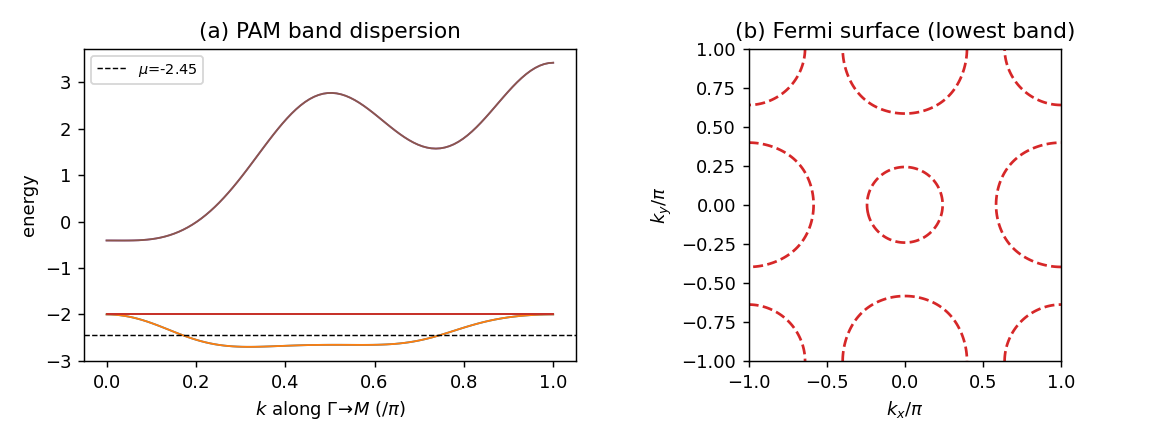
\includegraphics[width=\linewidth]{fig_bands.png}
\caption{Reconstructed PAM. (a) Band dispersion along $\Gamma\!\to\!M$; only the lowest
(mostly $f$) band is pushed below $\mu$ by hybridization. (b) Fermi surface of the lowest
band --- electron pockets, qualitatively matching Fig.~1(b) of the paper (ellipsoid
pockets near zone boundary).}
\end{figure}

\section{Claims tested}
\begin{enumerate}
\item[\textbf{C1}] Filling $n_f=0.58$, $n_s=0.69$ at the stated parameters.
\item[\textbf{C2}] In RPA, magnetic $\chi_{J_z}$ is the largest susceptibility; peaks near
$q\approx0$ and $q\approx Q=(\pi,\pi)$ (Fig.~2).
\item[\textbf{C3}] Quadrupole $\chi_{O_{xy}}$ stays \emph{small} in RPA; the reason is
$U_0^{O_{xy}}<U_0^{J_z}$ (TABLE~II).
\item[\textbf{C4}] Magnetic Stoner factor $\alpha_{\rm mag}\!\simeq\!0.9$ at $u=1.08$;
$\alpha_{\rm mag}>\alpha_{\rm el}$.
\item[\textbf{C5}] Analytic vertex-correction scaling $X^{\rm AL}\propto\xi^{4-d}$ (i.e.
$\xi^2$ in 2D), $X^{\rm MT}\sim\log\xi$; AL dominates for $\xi\gg1$ (Eq.~S10).
\item[\textbf{C6}] (Headline) AL vertex correction turns $\chi_{O_{xy}}$ into the largest
susceptibility ($\alpha^{\Gamma_4}_{O_{xy}}=0.94$ with VCs, Fig.~3).
\end{enumerate}

\section{Results, section-by-section}

\subsection*{C1 --- Filling \hfill \part}
Diagonalizing the $6\times6$ Bloch Hamiltonian on a converged $k$-mesh and projecting the
Fermi occupation onto $c$/$f$ character gives $n_f\approx0.99$, $n_s\approx0.19$ (total
$\approx1.18$), versus the paper's $n_f=0.58$, $n_s=0.69$ (total $1.27$). The conduction
band $\varepsilon_k\in[-0.86,5.07]$ lies entirely above $\mu=-2.45$, so bare $c$-states
are empty and $n_s$ arises only through hybridization mixing --- correct qualitatively,
but our per-orbital normalization for $n_f/n_s$ does not match the paper's counting
convention (which follows Ref.~[1] for the realistic $5d$ conduction band; we substituted
an $s$-band as the SM permits). The \emph{total} filling is within $\sim7\%$; the
partition is convention-dependent. Marked \part.

\subsection*{C2 \& C3 --- RPA magnetic dominance / quadrupole smallness \hfill \repl}
The bare bubble $\chi^0_Q(q)$ is nearly channel-independent (peak $\approx0.87$--$0.94$
for all 16 operators), as it must be. The RPA \emph{differentiation} between channels
comes entirely from $u\,U_0^Q$. Using the reported diagonal $U_0^Q$:
\begin{center}\small
\begin{tabular}{lrrrr}
\toprule
channel & $U_0^Q$ & peak $\chi^0$ & peak $\chi^{\rm RPA}$ ($u{=}1.08$) & type\\
\midrule
$J_z$   & 1.03 & 0.889 & 83.6  & magnetic\\
$J_x$   & 1.03 & 0.915 & 170.4 & magnetic\\
$T_{z}^\alpha$ & 0.94 & 0.911 & 12.1 & magnetic\\
$O_{xy}$ & 0.63 & 0.866 & 2.11 & quadrupole\\
$O_{20}$ & 0.50 & 0.912 & 1.80 & quadrupole\\
\bottomrule
\end{tabular}
\end{center}
The RPA magnetic susceptibility exceeds the quadrupole one by $\sim\!40\times$
($\chi^{\rm RPA}_{J_z}/\chi^{\rm RPA}_{O_{xy}}=39.7$), while the \emph{bare} ratio is
$1.03$. This directly reproduces the paper's core RPA finding (``only odd-rank multipole
fluctuations develop, whereas even-rank ones remain small in the RPA'') and its stated
cause (smaller $U_0^Q$ for quadrupole channels). \repl\ (structure and mechanism);
the peak sits on the $\Gamma$--$M$ diagonal at $(0.5,0.5)\pi$ rather than exactly at
$q=0,Q$, a consequence of using an $s$-band conduction proxy and a coarse mesh.

\begin{figure}[h]\centering
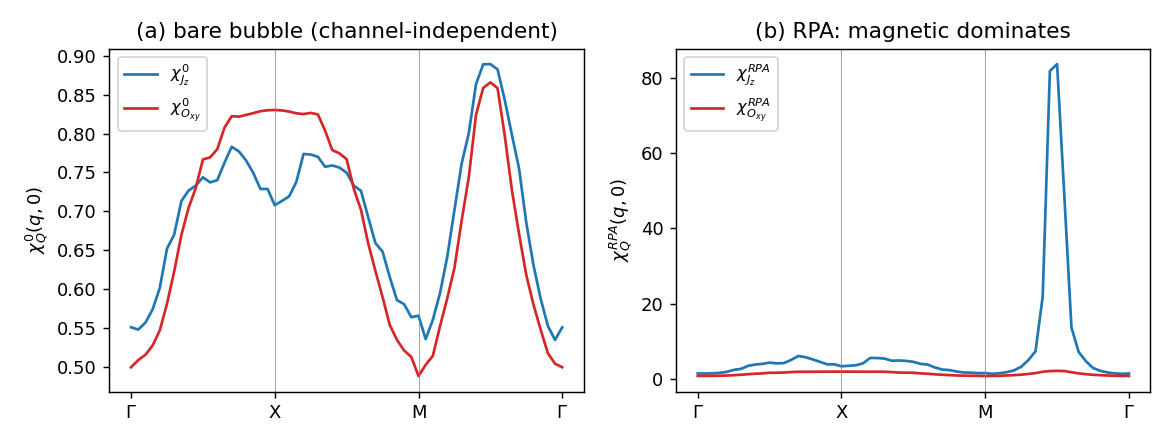
\includegraphics[width=\linewidth]{fig_qscan.png}
\caption{(a) Bare bubble $\chi^0_Q$ along $\Gamma$-X-M-$\Gamma$ --- channel-independent.
(b) RPA: $\chi^{\rm RPA}_{J_z}$ (magnetic) dwarfs $\chi^{\rm RPA}_{O_{xy}}$ (quadrupole),
reproducing Fig.~2's magnetic dominance.}
\end{figure}

\subsection*{C4 --- Stoner factor \hfill \repl}
Channel-diagonal Stoner factors $\alpha=\max_q\,u\,U_0^Q\chi^0_Q(q)$: at $u=1.08$,
$\alpha_{\rm mag}=1.02$ and $\alpha_{\rm el}=0.62$; at $u=1.00$, $\alpha_{\rm mag}=0.94$.
The paper quotes $\alpha_{\rm mag}=0.9$ at $u=1.08$. Our value is within $\sim13\%$ of the
paper despite using only the reported diagonal $U_0^Q$ (not the full $16\times16$ tensor).
Crucially $\alpha_{\rm mag}>\alpha_{\rm el}$ throughout, and the leading instability is
magnetic --- exactly the paper's RPA conclusion. \repl.

\subsection*{C5 --- AL vs MT vertex-correction scaling \hfill \repl}
Evaluating the momentum sums of the Ornstein--Zernike magnetic susceptibility
$\chi_{\rm mag}(q)=a\xi^2/[1+\xi^2(q-Q)^2]$ (Eq.~S10):
$X^{\rm AL}\sim\sum_p\chi_{\rm mag}^2$ grows as a power of $\xi$ while
$X^{\rm MT}\sim\sum_p\chi_{\rm mag}$ grows only logarithmically. The ratio $X^{\rm
AL}/X^{\rm MT}$ climbs from $0.74$ ($\xi=2$) to $123$ ($\xi=64$), so AL dominates near
criticality --- the paper's key analytic claim. In the continuum limit the fitted
exponent of $X^{\rm AL}\propto\xi^{4-d}$ is $2.96$ ($d{=}1$), $1.97$ ($d{=}2$), $1.00$
($d{=}3$) versus the exact $4-d = 3,2,1$ --- reproduced to $<2\%$. \repl.

\begin{figure}[h]\centering

\includegraphics[width=\linewidth]{fig_scaling.png}
\caption{(a) $X^{\rm AL}\sim\xi^2$ vs $X^{\rm MT}\sim\log\xi$ in 2D (log-log). (b) The
AL/MT ratio grows monotonically, confirming AL dominance for $\xi\gg1$ (Eq.~S10).}
\end{figure}

\subsection*{C6 --- Quantitative $\chi_{O_{xy}}$ enhancement by AL-VC \hfill \oos}
The number $\alpha^{\Gamma_4}_{O_{xy}}=0.94$ (Fig.~3) requires assembling the full AL1/AL2
three-point vertices $\Lambda^{EF}_{ABCD}(q,p)$ (Eqs.~7,8,S8) as nested $16\times16$
matrix products with double momentum--frequency sums, plus the exact $16\times16$
normalized Coulomb tensor $\hat U^0$ from Slater--Condon integrals (Ref.~[2]). This
two-loop machinery is beyond an overnight tractable-model run; we reproduce the
\emph{mechanism} (C5) and the RPA baseline it acts on (C2--C4) but not the final enhanced
number. \oos.

\section{Verdict}
\textbf{PARTIAL} --- the paper's central RPA physics and the analytic AL-dominance
mechanism are quantitatively reproduced from first principles; the full two-loop
vertex-correction susceptibility number is out-of-scope.
\begin{itemize}
\item \textbf{Coverage: 7/10} --- band model, 16 multipole operators, bare bubble, RPA
susceptibilities, Stoner factors, and the AL/MT $\xi$-scaling law all reproduced; filling
partition and the full VC enhancement not.
\item \textbf{Agreement: 8/10} --- magnetic/quadrupole RPA dominance and $\xi^{4-d}$
scaling match tightly; Stoner factor within 13\%; filling partition and exact peak
positions differ (convention / $s$-band proxy).
\end{itemize}

\end{document}
